\newpage
\section{Navigatore}
\label{sec:chapter_prove_sperimentali_navigator}

I test effettuati sul navigatore hanno permesso di osservare i benefici ottenuti nella fluidità di fruizione di una scena processata tramite il processo di  bake.
\\
In particolare sono stati effettuati dei confronti diretti tra la frequenza di fotogrammi al secondo proiettabili su schermo durante la renderizzazione di una scena con sole lightmap (senza fonti di luminose) e la frequenza durante il rendering di una scena non processata con il bake (con luci).
La presenza di luci, all’interno di una normale scena creata in Three.js, rappresenta uno dei maggiori fattori che incide sulle performance di renderizzazione e quindi sul numero di frame visualizzabili per secondo (fps).
\\
I confronti effettuati tra le due scene differenti, sopra descritte, hanno permesso di sperimentare quanto le luci incidano sulle prestazioni di rendering.
\\ 
Inoltre hanno permesso di valutare qualitativamente i miglioramenti visivi nella riproduzione delle fonti luminose ottenuti da un rendering di tipo Cycles rispetto ad uno di tipo Rasterization.
\subsection{Confronto prestazionale tra scena con o senza bake}
\label{sec:chapter_prove_sperimentali_navigator_confronto_prestazionale}
Il test effettuato prevede di sperimentare i benefici prestazionali, osservabili durante l’utilizzo del navigatore, di una scena che ha subito il processo di bake (senza luci) rispetto ad una non processata tramite il servizio bake (con luci).
\\
Il numero di luci di quest’ultima scena viene aumentato gradualmente per permettere di verificare come l’incremento di queste possa incidere sulle performance complessive del sistema. 
Infine i risultati di fluidità sperimentati vengono confrontati con le performance ottenibili dall’utilizzo di una scena senza luci con applicate le lightmap.
\\
Siccome questo test è fortemente dipendente dall’architettura utilizzata, esso viene effettuato su tre differenti architetture, rispettivamente, con prestazioni basse, medie ed alte.
\\
Nel dettaglio ogni test prevede di calcolare il numero di fotogrammi al secondo erogati dal navigatore durante la renderizzazione di cinque scene identiche per composizione di oggetti ma differenti per numero di luci inserite :5, 10, 20, 30 o 50 luci.
\\
Questi valori sono stati scelti in quanto per la realizzazione di un appartamento di media grandezza sono necessari solitamente un numero di luci comprese tra le dieci e le trenta; numero che raramente supera cinquanta.
\\
Le luci inserite risultano identiche per valori di intensità e per ampiezza dell’angolo luminoso (36 gradi). 
L’angolo luminoso in particolare è il parametro che maggiormente incide sulle prestazioni di rendering; per tutte le luci presenti nelle cinque scene è stato utilizzato il valore di 36 gradi.
\\
Questo valore rappresenta un tipo di angolazione che ben approssima l’angolo di luce di una lampada presente in un appartamento.
Nulla però esclude all’utilizzatore del servizio, creato in questo lavoro di tesi, di utilizzare luci con una elevata ampiezza dell’angolo luminoso.
\\ 
Quindi per ogni test è stata effettuata una ulteriore prova atta a valutare la fluidità di una sesta scena, identica a quella con 30 luci, in cui però ad ogni luce viene assegnato un valore di ampiezza angolare maggiore: 180 gradi.
\\
I sei risultati di fluidità provenienti dalle scene con luci vengono quindi confrontati con la frequenza di fotogrammi al secondo (fps) erogabili durante la renderizzazione di una scena (senza luci) processata tramite bake. Questa scena, con applicate le lightmap (senza luci), viene ottenuta dando in input al servizio di bake la scena con 50 luci.
Gli fps di ogni ambiente creato vengono calcolati sia per la vista dall’alto sia per quella in prima persona.
\\
Questo test ha permesso di sperimentare quanto effettivamente le luci incidano sulle performance di rendering e di comprendere a fondo in quali circostanze la tecnica di bake comporti i maggiori benefici in termini di prestazioni.
\\
Vengono adesso presentati i risultati di performance ottenuti su un calcolatore di fascia bassa con la seguente architettura:
\begin{itemize}
\item Processore: 2,4 GHz Intel Core 2 Duo.
\item Scheda grafica: NVIDIA GeForce 320M 256 MB.
\item Memoria RAM: 4 GB
\end{itemize}

La scena processata tramite il servizio di bake ha permesso di ottenere un frame rate stabile a 60 frame al secondo sia durante la navigazione dall'alto sia durante quella in prima persona.
I risultati della scena senza bake all'aumentare del numero di luci inserite sono invece descritti in tabella \ref{table:luci_basse_prest}

\begin{table}[]
\centering
\caption{Numero di luci e fluidità (architettura 1).}
\begin{tabular}{|l|l|l|l|}
\hline
\multicolumn{1}{|c|}{\textbf{\begin{tabular}[c]{@{}c@{}}numero\\ spotlight\end{tabular}}} & \multicolumn{1}{c|}{\textbf{\begin{tabular}[c]{@{}c@{}}angle\\ spotlight\end{tabular}}} & \multicolumn{1}{c|}{\textbf{\begin{tabular}[c]{@{}c@{}}frame-rate\\ dall'alto\end{tabular}}} & \multicolumn{1}{c|}{\textbf{\begin{tabular}[c]{@{}c@{}}frame-rate\\ prima persona\end{tabular}}} \\ \hline
5 & 36 & 28-40 & 29-35 \\ \hline
10 & 36 & 18-30 & 22-30 \\ \hline
20 & 36 & 20-25 & 16-25 \\ \hline
30 & 36 & 10-15 & 13-20 \\ \hline
30 & 180 & 7-12 & 9-13 \\ \hline
50 & 36 & 8-13 & 6-12 \\ \hline
\end{tabular}
\label{table:luci_basse_prest}
\end{table}

Dai risultati ottenuti è possibile osservare come la renderizzazione di una scena che non è stata processata tramite bake appesantisca il processo di rendering anche inserendo poche luci con ampiezza angolare di 36 gradi.
\\
La navigazione in prima persona risulta infatti problematica già quando nella scena sono inserite 5 fonti luminose. I più bassi valori di fps vengono raggiunti quando sono osservate più fonti luminose insieme.
\\
Con l’inserimento di un numero maggiore di 20 luci, la navigazione invece risulta impossibile; gli fps sono talmente bassi da non rendere fluida la scena.
\\
Nel caso di 50 luci sono inoltre presenti frequenti casi di blocco totale della navigazione con picchi che raggiungono 1 o 2 fps quando la camera è rivolta verso le luci.
La scena creata con 30 luci di ampiezza 180 gradi risulta identica in termini di fluidità a quella con 50 luci con ampiezza 36 gradi. 
\\
Risulta chiaro quindi come il valore di ampiezza incida pesantemente sulle performance di navigazione.
\\
La scena processata tramite il bake ha mantenuto invece un frame rate costante e vicino ai 60 fps durante la navigazione dall’alto ed un frame rate maggiore a 40 frame durante la navigazione in prima persona. Per entrambi i casi il frame rate è diminuito solamente in rari casi. Diminuzione di fluidità dovuta però dalla complessità degli oggetti renderizzati in quel momento dalla camera e non dal numero di luci.
\\
Risulta chiaro quindi che la scena processata tramite il servizio di bake permetta di migliorare notevolmente le prestazioni di rendering, comportando una maggiore fluidità generale nella fruizione della scena. 
\\
Adesso vengono presentati i risultati di performance ottenuti su un calcolatore di fascia media con la seguente architettura:
\begin{itemize}
\item Processore: Intel Core i7 - 3630QM 2.4GHZ.
\item Scheda grafica: NVIDIA GeForce GT635M 2GB.
\item Memoria RAM: 8 GB
\end{itemize}

La scena processata tramite il servizio di bake, esattamente come con il calcolatore di fascia bassa, ha permesso di ottenere un frame rate stabile a 60 frame al secondo sia durante la navigazione dall'alto sia durante quella in prima persona.
I risultati della scena senza bake all'aumentare del numero di luci inserite sono descritti in tabella \ref{table:luci_alte_prest} 
\begin{table}[h]
\centering
\caption{Numero di luci e fluidità (architettura 2).}
\begin{tabular}{|l|l|l|l|}
\hline
\multicolumn{1}{|c|}{\textbf{\begin{tabular}[c]{@{}c@{}}numero\\ spotlight\end{tabular}}} & \multicolumn{1}{c|}{\textbf{\begin{tabular}[c]{@{}c@{}}angle\\ spotlight\end{tabular}}} & \multicolumn{1}{c|}{\textbf{\begin{tabular}[c]{@{}c@{}}frame-rate\\ dall'alto\end{tabular}}} & \multicolumn{1}{c|}{\textbf{\begin{tabular}[c]{@{}c@{}}frame-rate\\ prima persona\end{tabular}}} \\ \hline
5 & 36 & 43-60 & 56-60 \\ \hline
10 & 36 & 37-41 & 46-60 \\ \hline
20 & 36 & 22-26 & 25-57 \\ \hline
30 & 36 & 17-18 & 17-51 \\ \hline
30 & 180 & 11-13 & 13-34 \\ \hline
50 & 36 & 12-14 & 12-32 \\ \hline
\end{tabular}
\label{table:luci_alte_prest}
\end{table}
Dai risultati ottenuti è possibile osservare come la renderizzazione nel navigatore di una scena che non è stata processata tramite bake risulti fluida in presenza di poche luci, con un frame rate elevato ma fortemente variabile.
Il frame rate esattamente come per il calcolatore di basse prestazioni risulta più basso quando la camera renderizza direttamente una o più luci.
Con l’inserimento di un numero maggiore di 20 luci la navigazione comincia a diventare problematica, con gli fps che subiscono un notevole decremento, e prosegue fino a risultare impossibile quando le luci raggiungono un numero vicino a 50.
Di fatto si ottiene una navigazione a scatti che alterna pochissimi momenti fluidi ad altri in cui essa risulta praticamente bloccata.
Esattamente come per l’archittettura con prestazioni più basse anche in questo caso la scena con 30 luci con ampiezza 180 ha prestazioni simili a quella in cui sono presenti 50 luci con piccola ampiezza.
Inoltre è possibile riscontrare come la vista dall’alto risulti per ogni scena generalmente meno fluida rispetto rispetto a quella in prima persona, questo perchè nella vista dall’alto vengo di solito renderizzate tutte le luci presenti nella scena.
\\
Invece la scena in cui è stato applicato il processo di bake è risultata fluida ed ha permesso di riscontrare un frame rate ancorato a 60 fps fissi sia per la vista dall’alto che per quella in prima persona.
\\
I risultati ottenuti in fase di sperimentazione hanno quindi confermato gli enormi vantaggi comportati dal renderizzare in ambiente web una scena processata mediante il servizio creato in questo lavoro di tesi.
Vantaggi che  migliorano all’aumentare del numero di luci inserite nella scena originale utilizzata come input nel processo.
\\
I risultati ottenuti hanno permesso di confermare il raggiungimento di uno degli obiettivi principali prefissati in questo lavoro di tesi e cioè rendere fruibile la scena anche su architetture meno performanti.
La scena ottenuta non solo è più leggere dal punto di vista computazionale del rendering ma è anche visivamente migliore.
Inoltre le sperimentazioni effettuate hanno permesso di osservare come i benefici di fluidità ottenuti siano maggiori all'aumentare del numero di oggetti luce inseriti nella scena originale.
Nel paragrafo seguente verranno presentati i miglioramenti visivi ottenuti dalle scene, altro obiettivo principale della tesi.

\subsection{Confronto qualitativo tra scena prima e dopo il bake}
In questo paragrafo vengono presentati i risultati visivi della scena ottenuta dal processo di bake. Quest’ultima viene confrontata con la scena creata in Three.js in cui non sono state applicate sole lightmap.
Questo confronto diretto permette di verificare i miglioramenti ottenuti nella riproduzione di luci ed ombre all’interno delle scene create tramite il servizio.
Inoltre permette di testare, a fronte del miglioramento, il grado di fedeltà tra le due scene prese in esame. Fedeltà ottenuta tramite la mappatura dei parametri di rendering Three.js-Blender creata nel presente lavoro di tesi.
\\
In particolare vengono qui proposti i risultati visivi ottenuti dal processo di bake di una scena che ricrea un appartamento reale.
La scena con applicate le lightmap ha impiegato 9 ore e 57 minuti di tempo per essere processata dal servizio; il valore di sampling utilizzato è stato 300.
\\
\begin{figure}[htb]
 \centering
 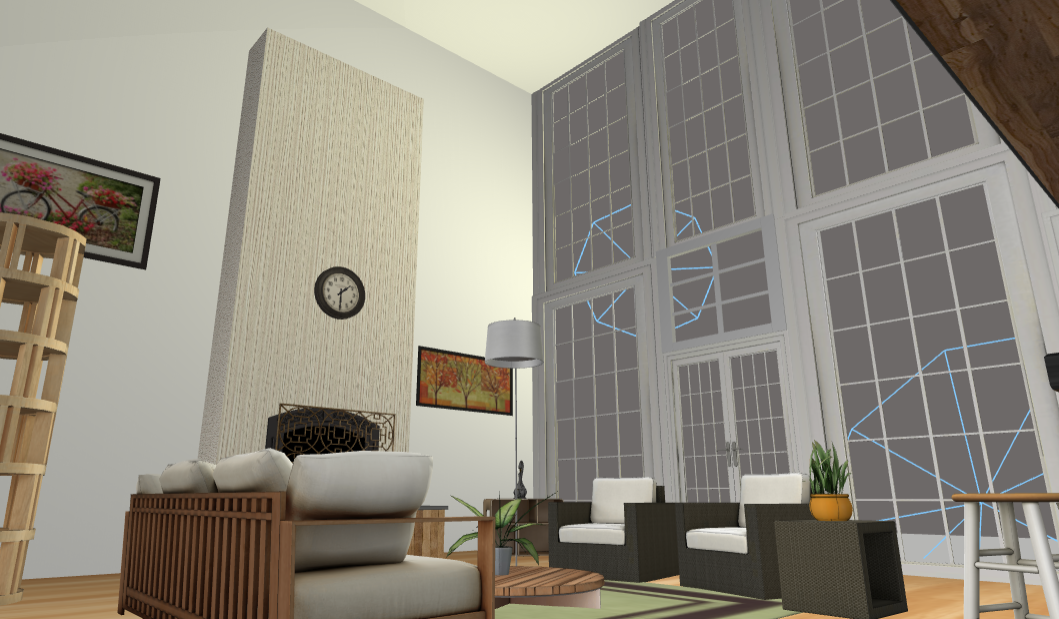
\includegraphics[width=0.8\linewidth]{images/chapter_prove_sperimentali/salone_vetrata_nobake.png}\hfill
 \caption[Salone senza lightmap, veduta 1]{Immagine del salone senza lightmap, veduta 1}
 \label{fig:prove_sperimentali_navigatore_vetrata_nobake}
\end{figure}
\\
\begin{figure}[h]
 \centering
 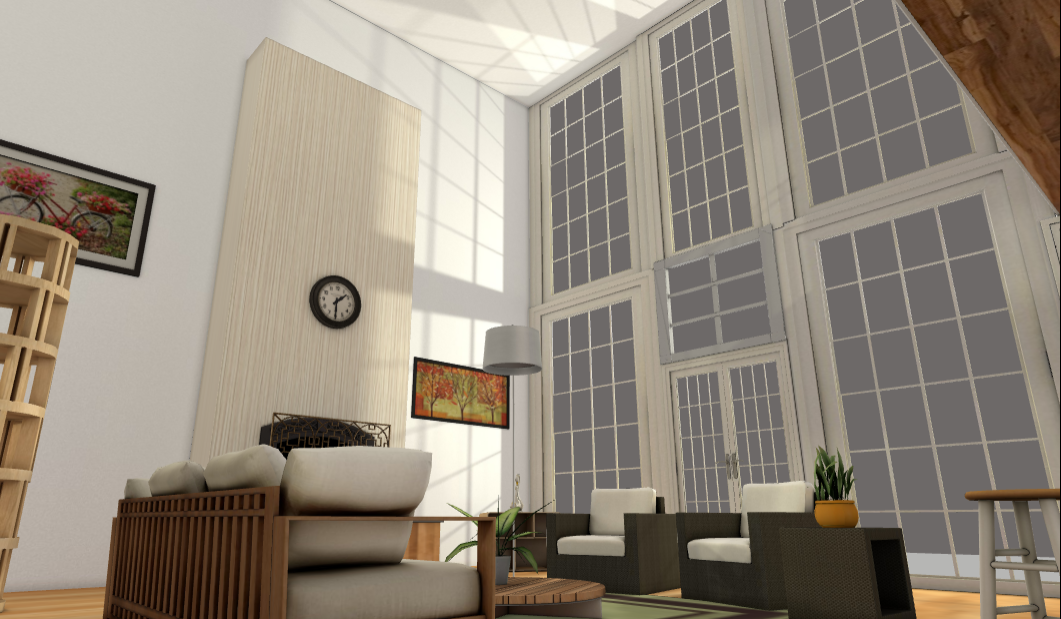
\includegraphics[width=0.8\linewidth]{images/chapter_prove_sperimentali/salone_vetrata_bake.png}\hfill
 \caption[Salone con lightmap, veduta 1]{Immagine del salone con lightmap, veduta 1}
 \label{fig:prove_sperimentali_navigatore_vetrata_bake}
\end{figure}
\\
Come visibile dalle immagini, nella scena processata con il bake sono mappate luci ed ombre estremamente realistiche.
Inoltre è possibile notare come le due luci visibili nella scena creata in Three.js (fig: \ref{fig:prove_sperimentali_navigatore_vetrata_nobake}) vengano correttamente mappate dal servizio di baking permettendo di ricreare la luce solare proveniente dall’esterno delle fineste (fig:\ref{fig:prove_sperimentali_navigatore_vetrata_bake}).
Inoltre è possibile notare come la luce sfumi di intensità mano a mano che entra all’interno dell’abitazione, effetto non riproducibile dal Rasterization Render.
\\
\begin{figure}[htb]
 \centering
 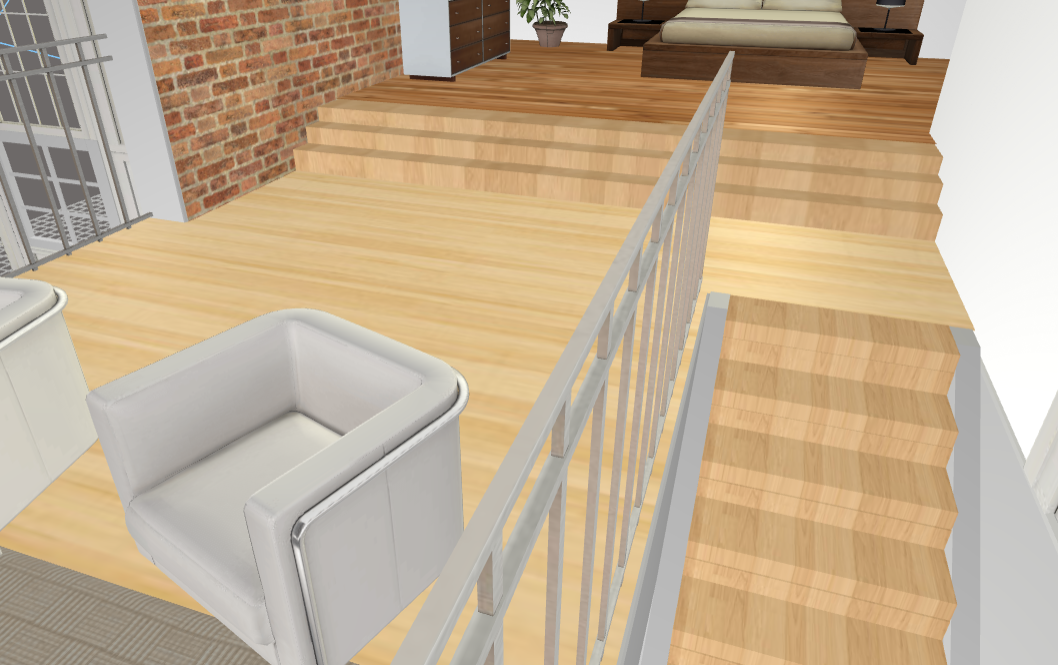
\includegraphics[width=0.8\linewidth]{images/chapter_prove_sperimentali/salone_scale_nobake.png}\hfill
 \caption[Salone senza lightmap, veduta 2]{Immagine del salone senza lightmap, veduta 2}
 \label{fig:prove_sperimentali_navigatore_scale_nobake}
\end{figure}
\\
\begin{figure}[htb]
 \centering
 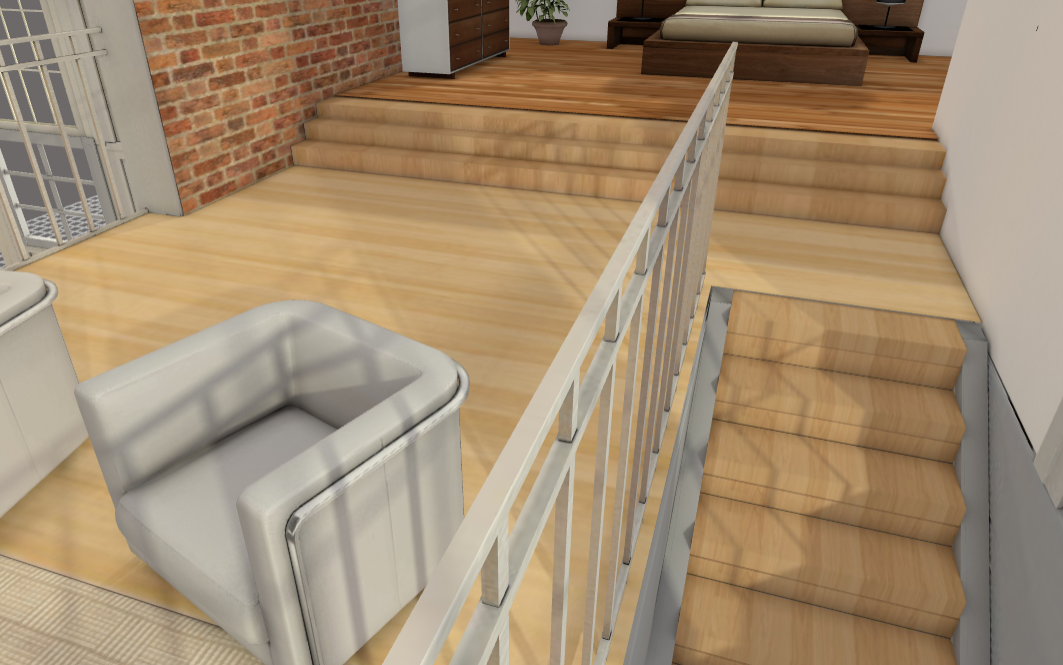
\includegraphics[width=0.8\linewidth]{images/chapter_prove_sperimentali/salone_scale_bake.png}\hfill
 \caption[Salone con lightmap, veduta 2]{Immagine del salone con lightmap, veduta 2}
 \label{fig:prove_sperimentali_navigatore_scale_bake}
\end{figure}
\\
Ulteriore confronto atto a mostrare i miglioramenti nel realismo della scena ottenuti tramite questo lavoro di tesi.
La fonte luminosa in questa scena è posizionata in basso a destra dell’immagine ed è rivolta verso l’appartamento. In questa foto è possibile osservare la riproduzione di ombre che sono ben definite quando vicino alla fonte luminosa e diventano più leggere con l’allontanarsi da essa.
Anche in questo caso è possibile notare come la mappatura dei parametri del servizio di bake abbia permesso di ricreare una scena fedele all’originale: per oggetti, colori, texture e luci.
\\
\begin{figure}[htb]
 \centering
 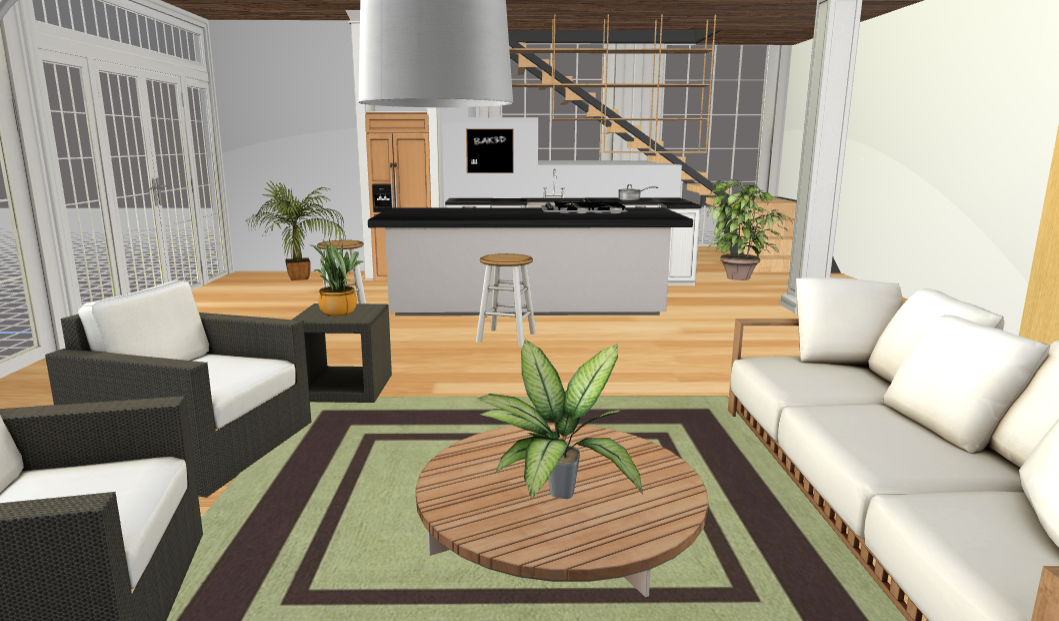
\includegraphics[width=0.8\linewidth]{images/chapter_prove_sperimentali/salone_camino_nobake.png}\hfill
 \caption[Salone senza lightmap, veduta 3]{Immagine del salone senza lightmap, veduta 3}
 \label{fig:prove_sperimentali_navigatore_scale_nobake}
\end{figure}
\\
\begin{figure}[htb]
 \centering
 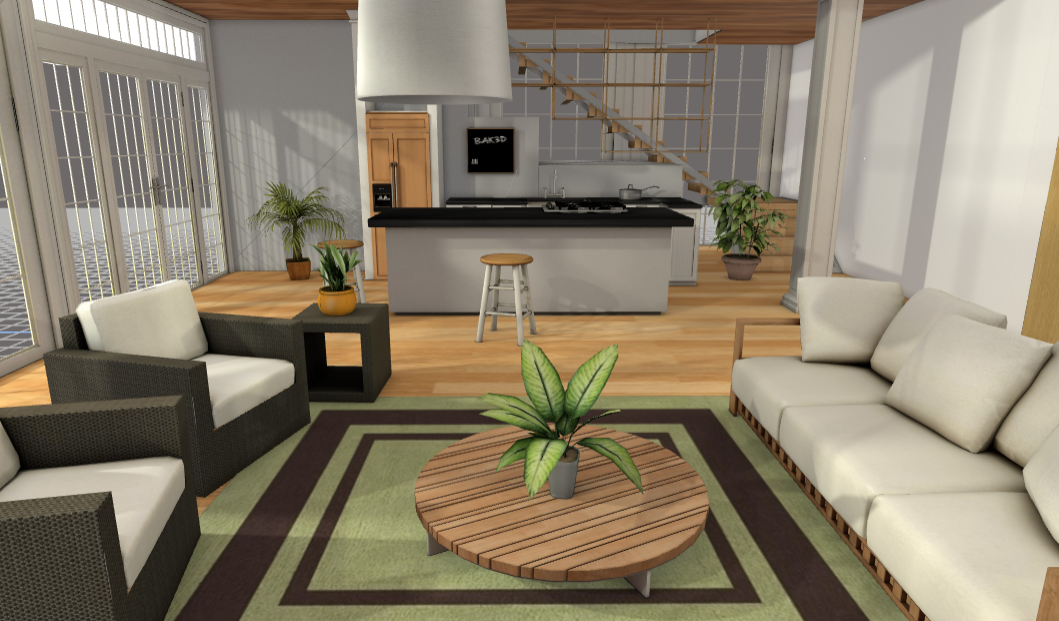
\includegraphics[width=0.8\linewidth]{images/chapter_prove_sperimentali/salone_camino_bake.png}\hfill
 \caption[Salone con lightmap, veduta 3]{Immagine del salone con lightmap, veduta 3}
 \label{fig:prove_sperimentali_navigatore_scale_bake}
\end{figure}
\\
Nella foto scattata dalla scena con il bake è possibile notare come il servizio abbia permesso la creazione di ombre appena distinguibili che si dissolvono verso i bordi. 
Questo tipo di ombre estremamente realistiche vengono chiamate soft shadow e sono impossibili da ricreare con il Rasterization render di Three.js. 
\\
In questo paragrafo sono stati quindi presentati i miglioramenti ottenuti nella creazioni di luci ed ombre. Miglioramenti che hanno permesso di aumentare notevolmente il grado di realismo delle scene create con il motore di rendering Three.js.
Inoltre queste scene risultino più leggere da renderizzare in quanto l’applicazione delle lightmap permette di rimuovere completamente dalla scena ogni tipo di fonte luminosa.
Ombre e luci fotorealistiche non risultano però l’unico miglioramento visivo applicato in questo lavoro di tesi.
\\
Nel paragrafo \ref{sec:chapter_prove_sperimentali_qualita_visiva} verranno infatti presentati i risultati visivi ottenuti aggiungendo alle scene create anche le envmap che hanno permesso la creazione di effetti di riflessione e rifrazione.

\subsection{Confronto prestazionale tra Three.Mirror ed envmap}
\label{sec:chapter_prove_sperimentali_mirror_envmap}
Il test effettuato prevede di valutare i benefici prestazionali ottenuti nella renderizzazione di una scena che utilizza envmap per gli effetti di riflessione rispetto ad una che utilizza l’oggetto Three.Mirror.
\\
In particolare viene valutata come varia la fluidità della navigazione in prima persona all’incrementare del numero di envmap ed all’incrementare del numero di Three.Mirror.
\\
Per questo test è stata utilizzato un portatile con una architettura di fascia bassa al fine di sperimentare la fluidità degli effetti di riflessione su un tipo di hardware accessibile a tutti.
\\
Il calcolatore utilizzato presenta la seguente architettura:
\begin{itemize}
\item Processore: 2,4 GHz Intel Core 2 Duo.
\item Scheda grafica: NVIDIA GeForce 320M 256 MB.
\item Memoria RAM: 4 GB
\end{itemize}
Nel dettaglio il test prevede la creazione di due scene identiche, una costituita da soli Three.Mirror e l’altro da sole envmap.
\\
Nella prima scena vengono calcolati il numero di fotogrammi al secondo erogati durante la navigazione all’aumentare del numero di Three.Mirror, da due a sette.
\\
Nella seconda vengono invece valutati gli fps all’ aumentare del numero delle env-map, anche in questo caso da due a sette.
\\
Al variare del numero di oggetti Three.Mirror nella prima scena i risultati ottenuti sono stati i seguenti:
\begin{table}[h]
\centering
\caption{Three.Mirror e fluidità (architettura 1).}
\begin{tabular}{|c|c|}
\hline
\textbf{Three.mirror} & \textbf{frame-rate} \\ \hline
2 & 36-40 \\ \hline
3 & 28-30 \\ \hline
4 & 15-24 \\ \hline
5 & 17-18 \\ \hline
6 & 15-17 \\ \hline
7 & 14-17 \\ \hline
\end{tabular}
\label{table:three_mirror}
\end{table}
Come osservabile anche solo l’inserimento di due specchi incide pesantemente sulle performance di renderizzazione e quindi sulla fluidità di navigazione.
\\
Navigazione che diventa impossibile già dopo l’inserimento di quattro specchi.
Bisogna però sottolineare come nella scena, creata per questo test, vengano inseriti un numero ristretto di oggetti (al massimo sette).
\\
Inserire infatti anche un solo oggetto Three.Mirror all’interno di una scena con molti oggetti, come gli interni creati per questo elaborato, abbasserebbe enormemente il valore frame rate al di sotto di dieci.
\\
Invece al variare del numero di envmap nella seconda scena i risultati ottenuti sono stati i seguenti:
\begin{table}[h]
\centering
\caption{Env map e fluidità (architettura 1).}
\begin{tabular}{|c|c|}
\hline
\textbf{Three.mirror} & \textbf{frame-rate} \\ \hline
2 & 36-40 \\ \hline
3 & 28-30 \\ \hline
4 & 15-24 \\ \hline
5 & 17-18 \\ \hline
6 & 15-17 \\ \hline
7 & 14-17 \\ \hline
\end{tabular}
\label{table:env-map}
\end{table}
Come osservabile il numero di fotogrammi al secondo si è mantenuto costante sui 60 frame anche con l’inserimento di sette effetti di riflessione ottenuti tramite le envmap, fluidità che sarebbe stata impossibile da raggiungere utilizzando i Three.Mirror.
\\
La tecnica delle env-map ha permesso inoltre di mantenere un frame rate ancorato sui 60 fino all’inserimento di 30 env-map dopodichè il frame-rate è improvvisamente sceso a 4,6 fps.
\\
Questa tecnica comporta quindi benefici enormi in termini di prestazioni ed è stata essenziale al fine di ottenere scene fotorealistiche navigabili anche su calcolatori di basse prestazioni o su smartphone e tablet
